\chapter{Evaluation} \label{chap:Evaluation}

  For all of the experiments the data was partitioned in a 50/50 split
  (by subject) as shown in table \ref{tab:splitting}:
  \begin{table}[h!]
    \centering { \footnotesize
    \begin{tabular}{|l|l|}
    \hline
    Set & Subjects   \\
    \hline
     Train          & 2,4,6,8,10,12,16,18,23,25,27,29,31      \\
    \hline
    Validation      & 1,3,5,7,9,11,13,17,21,24,26,28,30,32 minus test set     \\
    \hline
    Test           & 500 chosen randomly taken from validation set      \\
   \hline
    \end{tabular}
    \caption{The split of the DISFA dataset used in the experiments.}
    \label{tab:splitting} }
  \end{table}

  AU intensities 1-5 counted as a positive examples and AU intensity 0 counted as a negative example.
  To calculate autoencoder loss, ROC and F1 values for a trained model, the whole test
  set was run through the network and an average taken.

  To calculate the ROC the \texttt{sklearn} library was used, for the F1 20 thresholds
  between 0 and 1 were used and the best F1 score taken. For the autoencoder
  the losses were standardized by first applying the inverse transforms of the the preprocessing
  methods described in \ref{sec:methods} to the reconstructed images
  and then the mean squared difference was taken.

  \section{A Single Hidden Layer}

    To get a initial baseline reading of what the simplest model can achieve
    network \networkI\ is used. Per subject face normalisation from
    section \ref{sec:meanface} is chosen and the images are scaled with a factor of 1.0
    giving an image size $118 \times 118$.

    \begin{figure}[!h]
    \centering
    \includegraphics[width =\hsize]{../graphs/losses_2016_08_14_004.pdf}
    \caption{The losses of network \networkI\ during training. The $\alpha$ coefficient determines the balance between the
    classifier and the autoencoder losses, $\alpha=1$ signifies only autoencoder training
    while $\alpha=0$ means only classifier training. Over fitting is observed
    on all loss functions. Training the classifier
    overwrites the weights and hence ends up reducing
    the performance of the autoencoder however the
    model is so simple that the validation set remains almost constant.}
    \label{fig:simpleloss}
    \end{figure}

    Overfitting to the train set is evident very
    early in the training from figure \ref{fig:simpleloss},
    this occurs for a number of reasons:
    \begin{itemize}
      \item The model is very simple.
      \item The validation set might not fully represent many AUs and AU combinations possible.
      \item The train and validation sets have no subjects in common with the train set.
            So unless a subject independent model is learnt, a large degree of overfitting will always occur.
    \end{itemize}

    Training the classifier reduces the performance of the autoencoder on the
    training set visibly but interestingly the same is not true for the validation set, meaning
    that the autoencoder failed to learn a general hypotheses. This is
    excepted due to the simplicity of the model.

    \begin{table}[!h]
    \centering
    {\small
    \begin{tabular}{llllll}
    \hline
    \textbf{Class}    & \textbf{ROC} & \textbf{ROC Ranking} & \textbf{Max F1} & \textbf{Max Precision} & \textbf{Max Recall} \\ \hline
    1                 & 0.50  & fail  & 0.09  & 0.06    & 1.0      \\
    2                 & 0.60  & poor  & 0.07  & 0.05    & 1.0      \\
    4                 & 0.62  & poor  & 0.31  & 0.27    & 1.0      \\
    5                 & 0.49  & fail  & 0.02  & 0.02    & 1.0      \\
    6                 & 0.80  & fair  & 0.48  & 0.42    & 1.0      \\
    9                 & 0.46  & fail  & 0.11  & 0.06    & 1.0      \\
    12                & 0.89  & good  & 0.67  & 0.73    & 1.0      \\
    15                & 0.46  & fail  & 0.11  & 0.06    & 1.0      \\
    17                & 0.55  & fail  & 0.18  & 0.25    & 1.0      \\
    20                & 0.51  & fail  & 0.09  & 0.12    & 1.0      \\
    25                & 0.65  & poor  & 0.51  & 0.42    & 1.0      \\
    26                & 0.57  & fail  & 0.32  & 0.23    & 1.0      \\ \hline
    \textbf{Average:} & 0.59  & fail  & 0.25  & 0.22    & 1.0      \\ \hline
    \end{tabular} }
    \caption{The final evaluation for the training session shown in \ref{fig:simple}.
    AU 12 and 6 are the only AUs learnt well. These values were
    calculated on the test set. The maximum F1s, precisions and recalls
    were found by trying 20 threshold values between 0 and 1.}
    \label{tab:biglist}
    \end{table}

    Table \ref{tab:biglist} shows finally the scores for each AU, although as expected
    most AUs fail, this table shows the values that are normally averaged in the following sections
    and so is instructive to display early in the evaluation section.

  \clearpage
  \section{Joint Classification}
    Table \ref{tab:binsoftcomp} compares how each of the solutions from section \ref{sec:joints}
    perform in a network using mean face normalisation (not per subject) and using the network
    \networkII\
    , this network was chosen because it contains all of the
    main components of larger networks typically used for classification tasks,
    such as a convolutional layer, max pool layer and fully connected layer.
    % ID = 4 date = '2016_08_14' group = 'alpha'

    \begin{table}[!h]
        {\footnotesize
        \centering
        \begin{tabular}{lccc}
        \hline
        Final Layer   & Av. ROC &   Av. Best F1 &   Autoencoder Loss (Not normalised) \\
        \hline
        Binary Softmax Layers  &   0.73 &  0.34 &   20.7 \\
        Softmax Layer          &   0.69 &  0.30 &   15.8 \\
        Sigmoid Layer          &   0.50 &  0.19 &  126.2 \\
        \hline
        \end{tabular}
      \caption{Comparison of the three ways the final layer could be implemented
      using \networkII\ (see table \ref{tab:netII}). The
      preprocessing method used was face normalisation (not per subject).
      500 iterations were used. }
      \label{tab:binsoftcomp}
      }
      \end{table}

      The results show that the binary softmax layer outperforms the other
      solutions. The softmax layer is only slightly worse, but in order to
      accommodate for the potential of higher classification rates it is in
      theory also clear that the binary
      softmax is the better choice. This is because, in joint classification
      problems the simple softmax layer struggles to report more than 2 AUs as
      the outputs must add up to one. The low performance of the sigmoid layer
      is interesting and one reason might be that of vanishing gradients due to
      the bottleneck layer (which feeds into the final layer) containing high activation values.

      As the softmax layer is better in the results and has a better potential for good results
      it is chosen as the classifier for the following experiments.

      \section{Preprocessing methods} \label{sec:psearch}

          A comparison of the preprocessing methods from section
          \ref{sec:methods} and on the four main activation functions
          that are typically used on the last layer of an autoencoder
          (linear, ReLU, sigmoid and tanh) was performed,
          table \ref{tab:psearch} shows the results.

          These parameters cover a lot of possible
          configurations and should have markedly different results, the idea
          is that the encoding at the bottleneck layer should be different for
          each set of parameters and that
          one of these might offer a good starting set of weights for the
          classifier to train from. What is typically meant by this is, is that
          the autoencoder has learnt to pick out some useful features, which the classifier
          can then build on.

          \begin{table}[!h] {\footnotesize
            \centering
          \begin{tabular}{lllrrrrrr}
                && &   \multicolumn{3}{|c|}{Autoencoder Training} &  \multicolumn{3}{c|}{Classifier Training}    \\
            \hline
             i&Preprocessing    & Activation Function&  ROC&F1&AE Loss & ROC & F1 & AE Loss \\
             \hline
             1&Per Subject Contrast Face & linear &    0.49 &   0.19 &     0.12 &    0.82 &   0.46 &     0.18 \\
             2&Per Subject Contrast Face & tanh   &    0.49 &   0.19 &     0.12 &    0.82 &   0.46 &     0.13 \\
             3&Per Subject Contrast Face & relu   &    0.63 &   0.19 &     0.12 &    0.81 &   0.44 &     0.14 \\
             4& Per Subject Contrast Face & sigmoid &    0.52 &   0.2  &     0.13 &    0.08 &   0.19 &     0.13 \\
             \hline
             5&Contrast          & linear &    0.40 &   0.19 &     0.19 &    0.74 &   0.34 &     1.46 \\
             6&Contrast          & tanh   &    0.61 &   0.19 &     0.20 &    0.72 &   0.35 &     0.35 \\
             7&Contrast          & relu   &    0.59 &   0.19 &     0.25 &    0.75 &   0.36 &     0.65 \\
             8& Contrast         & sigmoid &    0.54 &   0.19 &     0.22 &    0.50    &   0.19 &     0.28 \\
             \hline
             9&Face              & linear &    0.46 &   0.19 &     0.06 &    0.73 &   0.35 &     0.26 \\
             10&Face              & tanh   &    0.52 &   0.19 &     0.08 &    0.74 &   0.35 &     0.13 \\
             11&Face              & relu   &    0.45 &   0.19 &     0.09 &    0.73 &   0.36 &     0.35 \\
             12& Face             & sigmoid &    0.47 &   0.2  &     0.1  &    0.72 &   0.35 &     0.13 \\
             \hline
             \hdashline
             13&Per Subject Face  & linear &    $0.64$ &   $0.19$ &     $0.03$ &    $0.83$ &   $0.48$ &     $0.12$ \\
             &{\it error:}  &&$\pm$0.02 &$\pm$0.01 &$\pm$0.02  &$\pm$0.02 &$\pm$0.01 &$\pm$0.02 \\
             \hdashline
             14&Per Subject Face  & tanh   &    0.56 &   0.19 &     0.03 &    0.81 &   0.47 &     0.05 \\
             15&Per Subject Face  & relu   &    0.56 &   0.19 &     0.04 &    0.81 &   0.48 &     0.11 \\
             16& Per Subject Face      & sigmoid &    0.62 &   0.23 &     0.04 &    0.81 &   0.46 &     0.05 \\
             \hline
             17&Range [-1,1]      & linear &    0.50 &   0.19 &     0.07 &    0.73 &   0.35 &     3.90 \\
             18&Range [-1,1]      & tanh   &    0.54 &   0.19 &     0.07 &    0.75 &   0.35 &     0.30 \\
             19&Range [-1,1]      & relu   &    0.48 &   0.19 &     0.15 &    0.73 &   0.35 &     4.73 \\
             20& Range [-1,1]      & sigmoid &    0.49 &   0.2  &     0.12 &    0.73 &   0.31 &     0.36 \\
             \hline
             21&None              & linear &    0.51 &   0.19 &     0.08 &    0.74 &   0.34 &     4.02 \\
             22&None              & tanh   &    0.59 &   0.19 &     0.07 &    0.71 &   0.33 &     0.93 \\
             23&None              & relu   &    0.53 &   0.19 &     0.20 &    0.53 &   0.23 &     0.41 \\
             24& None       & sigmoid &    0.47 &   0.19 &     0.09 &    0.65 &   0.29 &     0.46 \\
             \hline
             25&Contrast Face     & linear &    0.56 &   0.19 &     0.24 &    0.74 &   0.35 &     0.40 \\
             26&Contrast Face     & tanh   &    0.54 &   0.19 &     0.24 &    0.75 &   0.38 &     0.26 \\
             27&Contrast Face     & relu   &    0.54 &   0.19 &     0.25 &    0.74 &   0.35 &     0.35 \\
             28& Contrast Face    & sigmoid &    0.44 &   0.19 &     0.25 &    0.71 &   0.34 &     0.26 \\
             \hline
            \end{tabular}
              \caption{Comparison of four activation functions for the autoencoder for each type of preprocessing method.
              Error values are required because TensorFlow does implement fully deterministic
              processing with GPU cards (see section \ref{sec:GPU} the values in the errors were
              calculated by rerunning experiment 13 5 times. The autoencoder losses were calculated
              by first applying the inverse transform of the preprocessing method and then taking the mean squared
              difference between the reconstructed image and original image. {\bf Experimental Configuration:}
              The alpha function is $\alpha(t)=\alpha_{\text{step}}(t,0.5,1000)$.
              meaning the autoencoder training runs for 500 iterations and then the classifier for 500.
              The network used is \networkII.}
          \label{tab:psearch} }
          \end{table}

          No significant difference is seen between the activation functions apart from with the sigmoid
          which makes training the classifier fail completely.

          The highest ROC and F1 score is found in experiment 13 in table \ref{tab:psearch}. Experiment 12
          has effectively the same score and a lower final autoencoder loss, but it uses the tanh activation
          function and hence cannot fully reconstruct the input image which has values well outside the
          range $[-1,1]$ hence the linear activation function is chosen to ensure the potential for full reconstruction is there.
          Also since this preprocessing method tries to correlate high activation values with AU occurrences, these high values should be
          an important focus of the reconstruction, the tanh functions might focus more on the smaller values which
          do not encode as much AU information.

        %
        %
        %
        %
        %
        \newpage
        \section{Shared Weights}

          Table \ref{tab:sharedweights} shows
          for three networks the effect of having and not having shared weights.

          \begin{table}[!h] \centering
          {\footnotesize
          \begin{tabular}{rrllrrrrrrrr}
            &&&&   \multicolumn{3}{|c|}{Autoencoder Training} &  \multicolumn{3}{c|}{Classifier Training}    \\
          \hline
            i & Network               &   Shared Weights &    ROC&F1&AE Loss & ROC & F1 & AE Loss \\
          \hline
           1 & \networkII    & False     &    0.38 &   0.19 &     0.03 &    0.79 &   0.45 &     0.05 \\
           2 & \networkII    & True      &    0.48 &   0.19 &     0.02 &    0.81 &   0.48 &     0.12 \\
          \hline
          4 & \networkIII    & False     &    0.55 &   0.19 &     0.03 &    0.78 &   0.41 &     0.06 \\
          5 & \networkIII    & True      &    0.56 &   0.19 &     0.02 &    0.8  &   0.46 &     0.18 \\
          \hline
          8 & \networkIV     & False     &    0.54 &   0.19 &     0.03 &    0.77 &   0.38 &     0.05 \\
          9 & \networkIV     & True      &    0.42 &   0.19 &     0.03 &    0.78 &   0.42 &     1.37 \\
           \hline
         \end{tabular}}
             \caption{A simple experiment showing that using shared weights is beneficial
             to both autoencoder loss and classification performance. {\bf Experimental Configuration:}
             The alpha function is $\alpha(t)=\alpha_{\text{step}}(t,0.5,1000)$.
             meaning the autoencoder training runs for 500 iterations and then the classifier for 500.
             The network is described in table \ref{tab:netII}.} \label{tab:sharedweights}
         \end{table}

          It can be seen that using shared weights consistently improves the classification
          performance by a small amount and in some cases the autoencoder performance.
          This could for a number of reasons:
          \begin{itemize}
            \item The more constrained (few parameters) model acts as a good base for classification training
            \item The model learnt without shared weights resembles the identity function and hence is not useful for classification
          \end{itemize}

          In the case of shared weights, the classifier has influence on the weights
          inside of the decoder section, hence as expected in these cases the autoencoder
          is damaged.

          These finding suggest it is useful to include shared weights in a model.
        %
        %
        %
        %
        %
        \newpage
        \section{Local Contrast Normalisation}

          The local contrast normalisation (LRN) scheme
          as described in section \ref{sec:lrn}
          was applied to the three test networks.

          Since some networks can have more than one LRN layer, the effect of
          using some LRN deeper in the network is also tested.

          \begin{table}[!h] \centering
            \footnotesize{
            \begin{tabular}{rrllrrrrrrrr}
              &&&   \multicolumn{3}{|c|}{Autoencoder Training} &  \multicolumn{3}{c|}{Classifier Training}    \\
            \hline
              i & Network             & LRN Layers   &    ROC&F1&AE Loss & ROC & F1 & AE Loss \\
            \hline
             1 & \networkII & 0  &    0.48 &   0.19 &     0.02 &    0.81 &   0.48 &     0.12 \\
             2 & \networkII & 1  &    0.49 &   0.19 &     0.02 &    0.81 &   0.47 &     0.13 \\
            \hline
             3 & \networkIII & 0  &    0.56 &   0.19 &     0.02 &    0.8  &   0.46 &     0.18 \\
             4 & \networkIII & 1  &    0.57 &   0.19 &     0.02 &    0.8  &   0.46 &     0.19 \\
             5 & \networkIII & 2  &    0.52 &   0.19 &     0.02 &    0.8  &   0.45 &     0.22 \\
            \hline
             6 & \networkIV & 0  &    0.42 &   0.19 &     0.03 &    0.78 &   0.42 &     1.37 \\
             7 & \networkIV & 1  &    0.52 &   0.19 &     0.03 &    0.79 &   0.44 &     1.02 \\
             8 & \networkIV & 2  &    0.52 &   0.19 &     0.03 &    0.8  &   0.44 &     0.88 \\
            \hline
            \end{tabular}}

            \caption{Results for applying local contrast normalisation layers
            for the three test networks. LRN Layers 0 means no LRN, 1 means a LRN layer is added after the max pool
            and 2 means a LRN layer is added at the final convolutional layer in the encoder. There is no
            inverse for LRN and hence the decoder section remains unchanged. {\bf Experimental Configuration:} see caption
            for table \ref{tab:sharedweights}
            }
            \label{tab:lrn}
          \end{table}

          Table \ref{tab:lrn} shows that LRN provides some improvement in performance for network 4 and seems
          not to effect the other networks by much. It is interesting that the larger network
          is less likely to reduce autoencoder loss with the LRN layers.

          For these reasons, as LRN seems to improve the bigger networks performance it
          would be good to include in the final model.

          \newpage
        %
        %
        %
        %
        %
        %
        \newpage
        \section{Dropout}
          Varying degrees of dropout (see section \ref{sec:dropout}) were applied to each convolutional
          network at the bottleneck layer.
          Table \ref{tab:dropout} shows the results.
          \begin{table}[h]
          \centering
          { \footnotesize
          \begin{tabular}{rllrrrrrrrr}
                               &         &                                                                                   &                                                                                  & \multicolumn{1}{r|}{} & \multicolumn{3}{c|}{Autoencoder Training}                          & \multicolumn{3}{c|}{Classifier Training}                           \\ \hline
          i                    & network & \multirow{2}{*}{\begin{tabular}[c]{@{}l@{}}Autoencoder\\ Iterations\end{tabular}} & \multirow{2}{*}{\begin{tabular}[c]{@{}r@{}}Classifier\\ Iterations\end{tabular}} & Dropout                    & ROC                  & F1                   & AE Loss              & ROC                  & F1                   & AE Loss              \\
          \multicolumn{1}{l}{} &         &                                                                                   &                                                                                  & \multicolumn{1}{l}{}  & \multicolumn{1}{l}{} & \multicolumn{1}{l}{} & \multicolumn{1}{l}{} & \multicolumn{1}{l}{} & \multicolumn{1}{l}{} & \multicolumn{1}{l}{} \\ \hline
          1                    & \networkII       & 1000              & 500     & 1        & 0.49     & 0.19      & 0.02      & 0.8                  & 0.47                 & 0.12                 \\
          2                    & \networkII       & 1000             & 500       & 0.9      & 0.49     & 0.19      & 0.03      & 0.8                  & 0.47                 & 0.11                 \\
          3                    & \networkII       & 1000             & 500       & 0.8      & 0.52     & 0.19      & 0.03      & 0.82                 & 0.48                 & 0.08                 \\
          4                    & \networkII       & 1000             & 1000       & 0.8      & 0.52     & 0.19      & 0.03      & 0.8                  & 0.46                 & 0.11                 \\
          \hline
          5                    & \networkIII       & 1000             & 500       & 1        & 0.51     & 0.19      & 0.02      & 0.81                 & 0.46                 & 0.21                 \\
          6                    & \networkIII       & 1000             & 500       & 0.9      & 0.51     & 0.19      & 0.02      & 0.81                 & 0.46                 & 0.25                 \\
          7                    & \networkIII       & 1000             & 500       & 0.8      & 0.49     & 0.19      & 0.03      & 0.82                 & 0.46                 & 0.13                 \\
          6                    & \networkIII       & 1000             & 1000       & 0.8      & 0.57     & 0.19      & 0.02      & 0.81                 & 0.44                 & 0.33                 \\
          \hline
          9                    & \networkIV       & 1000             & 500       & 1        & 0.6      & 0.19      & 0.03      & 0.78                 & 0.42                 & 1.03                 \\
          10                   & \networkIV       & 1000             & 500       & 0.9      & 0.63     & 0.19      & 0.03      & 0.71                 & 0.35                 & 0.15                 \\
          11                   & \networkIV       & 1000             & 500       & 0.8      & 0.5      & 0.19      & 0.03      & 0.73                 & 0.36                 & 0.08\\
          12                   & \networkIV       & 1000             & 1000       & 0.8      & 0.52      & 0.19      & 0.03      & 0.77   & 0.38     & 1.01\\
          \hline
          \end{tabular}
          }
          \caption{12 experiments which investigate the affect of applying dropout to the
          three test networks, autoencoder iterations is how many iterations
          the autoencoder is trained for and classifier iterations is for how many
          iterations the
          classifier is then trained. The dropout value represents the
          fraction of neurons which are kept active in the bottleneck layer of each network.
          {\bf Experimental Configuration:} see caption for table \ref{tab:sharedweights}.}
          \label{tab:dropout}
          \end{table}

          All networks are trained with the same number of iterations but they are of very different sizes,
          hence this analysis should not be seen fully as a comparison between networks,
          but a comparison between different amounts of dropout for each network.

          More dropout had little effect on the ROC for networks 2 and 3, however it does
          improve the final loss of the autoencoder. For network 4 the dropout actually decreases
          ROC performance, but again allows the autoencoder to remain more functional.
          The fact that the autoencoder is protected
          agrees with the general idea that any form of regularisation will inhibit large changes
          in weights and encourage less complex models, i.e. it should be easier for the classifier to try and learn
          a representation based on what the autoencoder was doing, instead of replacing it with a completely unrelated
          representation. Another explanation is that the autoencoder
          actually learns a representation which is more helpful for the classifier. This second hypothesis is
          however difficult to prove from the results as the autoencoder losses seem to not be affected by the dropout rate.

          In fact the autoencoder loss seems to have saturated around 0.02-0.03 which
          is an interesting result.

          Experiments 4,6 and 12 show that networks 2 and 3 are almost fully
          trained with 500 iterations as adding more iterations does little
          (even reducing the performance somewhat, but not more than is
          statistically relevant because these values still in have an error).

          To conclude, dropout should be included in the final model as it improves
          classification performance in most cases.

        \newpage
        %
        %
        %
        %
        %
        %
        \section{L2 Regularisation}

          Table \ref{tab:l2_1} shows some experiments which vary $\beta$ (described in sections \ref{sec:modl2} and \ref{sec:bacl2}), they reveal an
          interesting trend, where the ROC and F1 are reduced by L2 losses but the autoencoding
          ability is protected by the L2 loss term. Furthermore the L2 loss term acts
          to bring the cross entropy losses (CEL) of the validation set and train set closer together as can be seen in the table.

          \begin{table}[!h] {\footnotesize \centering
          \begin{tabular}{lrrrrrrrrrrr}
              &&&   \multicolumn{3}{|c|}{Autoencoder Training} &  \multicolumn{5}{c|}{Classifier Training}  \\
            \hline
             i & $\beta$ &   Iterations &   ROC&F1&AE Loss & ROC & F1 & AE Loss &   Validation CEL &   Train CEL \\
            \hline
             1 &     0     & 1000 &    0.45 &   0.19 &     0.03 &    0.77 &   0.46 &     0.11 &  0.53 &  0.07 \\
             2 &     0.001 & 1000 &    0.56 &   0.19 &     0.03 &    0.74 &   0.41 &     0.05 &  0.46 &  0.11 \\
             3 &     0.01  & 1000 &    0.45 &   0.19 &     0.03 &    0.71 &   0.36 &     0.04 &  0.33 &  0.18 \\
             4 &     0.1   & 1000 &    0.54 &   0.19 &     0.04 &    0.66 &   0.28 &     0.04 &  0.3  &  0.26 \\
             5 &     0.5   & 1000 &    0.5  &   0.19 &     0.04 &    0.46 &   0.19 &     0.04 &  0.32 &  0.33 \\
            \hline
          \end{tabular}
            \caption{The experimental set up is the same as in section \ref{sec:psearch} where the preprocessing methods
            were tested, except a slightly earlier version
            of the code was used and hence different ROC and F1 numbers.
            The results should still hold relative to each other.
            CEL (Cross Entropy Loss) is included here to get an idea of how different
            the losses between the validation batches are (of course the
            train batch is just 100 frames, however inspecting figure \ref{fig:l2_1} shows that
            these 100 frames are typically representative enough to draw conclusions from), these
            CEL values are therefore equivalent to the final data points in figure \ref{fig:l2_1}. } \label{tab:l2_1}
          }
          \end{table}

        Table \ref{tab:l2_2} then takes experiments 1 and 4 from table \ref{tab:l2_1} and doubles
        the amount of iterations for both the autoencoder and classifier trainings. It shows
        that the extra iterations can undo the performance loss that the L2 regularisation
        introduces while also still protecting the functionality of the autoencoder.
        This shows in general that L2 is a helpful thing to include in the setting of the autoencoder
        and classifier.

        \begin{table}[!h]
          {\footnotesize \centering
          \begin{tabular}{lrrrrrrrrrrr}
            &&&   \multicolumn{3}{|c|}{Autoencoder Training} &  \multicolumn{3}{c|}{Classifier Training}    \\
          \hline
           i &   $\beta$ &   Iterations &   ROC&F1&AE Loss & ROC & F1 & AE Loss \\
          \hline
           1 &       0.1 & 2000 &    0.56 &   0.19 &     0.03 &    0.74 &   0.35 &     0.04\\
           2 &       0   & 2000 &    0.46 &   0.19 &     0.03 &    0.77 &   0.45 &     0.15\\
          \hline
        \end{tabular}
        \caption{Identical to \ref{tab:l2_1} except with more iterations to investigate what happens with further training.
        The autoencoder and classifier are both trained for 1000 iterations.}
        \label{tab:l2_2} }
        \end{table}

        \begin{figure}[!h]
          \centering
            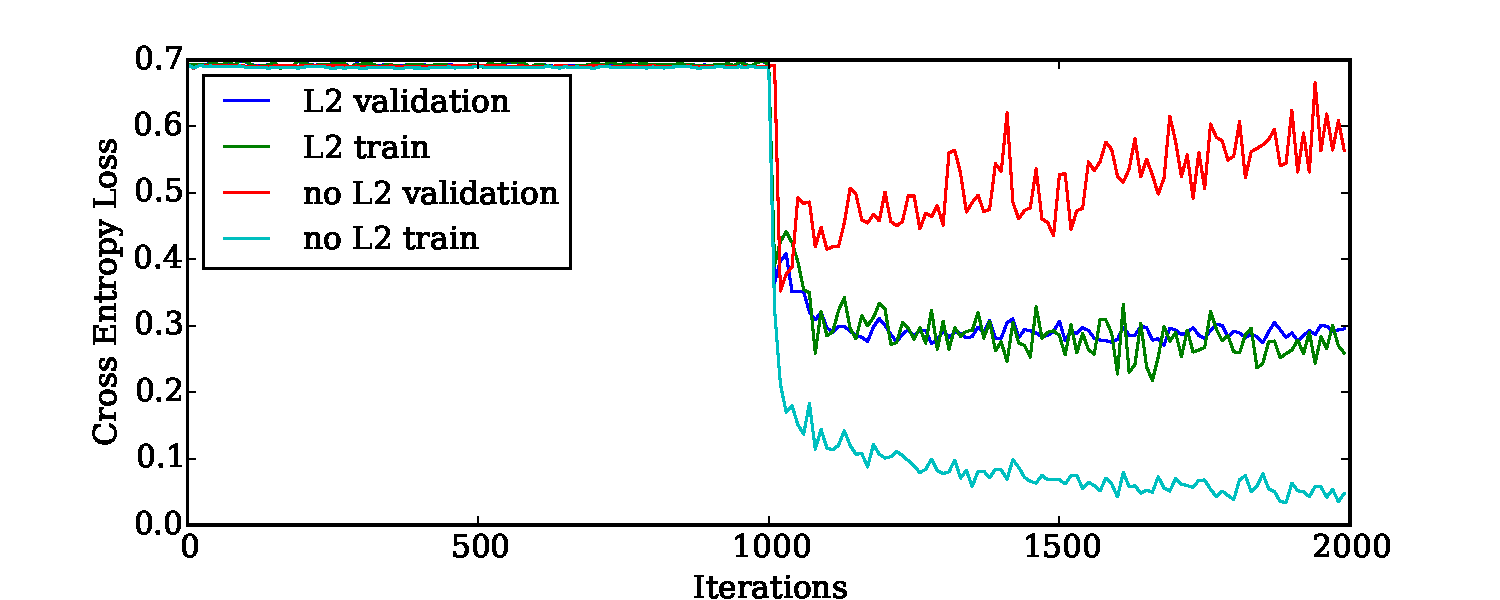
\includegraphics[width =0.8\hsize]{figures/l2.pdf}
              \caption{Plot of the classifier cross entropy losses of the two experiments in table \ref{tab:l2_2} during training.}
          \label{fig:l2_1}
        \end{figure}

        \begin{figure}[!h]
          \centering
            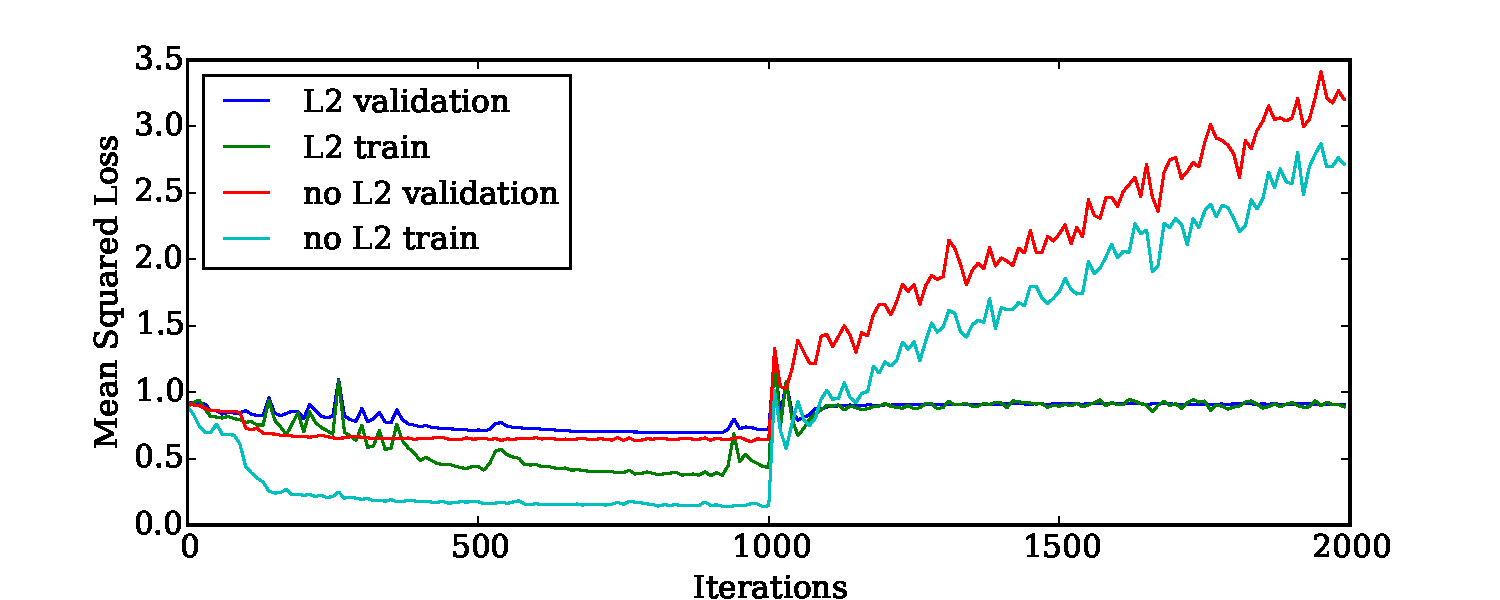
\includegraphics[width =0.8\hsize]{figures/l2_auto.pdf}
              \caption{Plot of the autoencoder mean squared loss of the two experiments in table \ref{tab:l2_2} during training.}
          \label{fig:l2_2}
        \end{figure}

        With these results then, the conclusion is that including a small degree of L2
        Regularisation should be useful for exploring the aims of this project.
        However as there is no significant improvement in classification performance
        and training takes longer it is not included in the final model.


        %
        %
        %
        %
        %
        %
      \section{Autoencoder classifier balancing functions}
        This section investigates the autoencoder balance functions described in section \ref{sec:autoalpha}.
        In addition to these, the classifier only ($\alpha(t) = 0$) are included as a baseline from which to compare
        what the autoencoder actually changes. The experimental question being asked here
        is whether the inclusion of the autoencoder can improve classification performance within the 1500 iterations
        that the network is trained for.



        \begin{table}[]
          \footnotesize{
          \centering
          \begin{tabular}{rrrrrrrrrrr}
                               &                      &                                                                              &                                                                              & \multicolumn{1}{r|}{}                                                       & \multicolumn{3}{c|}{Early Model}                                   & \multicolumn{3}{c|}{Final Model}                                   \\ \hline
          i                    & Network              & \multirow{2}{*}{\begin{tabular}[c]{@{}r@{}}Balance \\ Function\end{tabular}} & \multirow{2}{*}{\begin{tabular}[c]{@{}r@{}}Total \\ Iterations\end{tabular}} & \multirow{2}{*}{\begin{tabular}[c]{@{}r@{}}Early \\ Iteration\end{tabular}} & ROC                  & F1                   & AE Loss              & ROC                  & F1                   & AE Loss              \\
          \multicolumn{1}{l}{} & \multicolumn{1}{l}{} &                                                                              &                                                                              &                                                                             & \multicolumn{1}{l}{} & \multicolumn{1}{l}{} & \multicolumn{1}{l}{} & \multicolumn{1}{l}{} & \multicolumn{1}{l}{} & \multicolumn{1}{l}{} \\ \hline
          2.5                  & \networkII                    & constant 0.0         & 1500           & 1000    & 0.8   & 0.47 & 0.56  & 0.79 & 0.46 & 0.64  \\
          2.3                  & \networkII                    & constant 0.5         & 1500           & 750     & 0.81  & 0.48 & 0.03  & 0.8  & 0.46 & 0.03  \\
          2.1                  & \networkII                    & step                 & 1500           & 1000    & 0.59  & 0.19 & 0.03  & 0.82 & 0.47 & 0.08  \\
          2.4                  & \networkII                    & sigmoid              & 1500           & 1000    & 0.8   & 0.46 & 0.03  & 0.79 & 0.46 & 0.03  \\
          2.6                  & \networkII                    & polynomial           & 1500           & 750     & 0.79  & 0.46 & 0.03  & 0.77 & 0.44 & 0.03  \\
          2.2                  & \networkII                    & alternate            & 1500           & 1000    & 0.81  & 0.46 & 0.1   & 0.82 & 0.47 & 0.12  \\
          \hline
          3.5                  & \networkIII                   & constant 0.0         & 1500           & 1000    & 0.81  & 0.43 & 2.38  & 0.79 & 0.42 & 2.61  \\
          3.2                  & \networkIII                   & constant 0.5         & 1500           & 750     & 0.81  & 0.46 & 0.03  & 0.81 & 0.46 & 0.03  \\
          3.1                  & \networkIII                   & step                 & 1500           & 1000    & 0.38  & 0.19 & 0.03  & 0.81 & 0.45 & 0.18  \\
          3.3                  & \networkIII                   & sigmoid              & 1500           & 1000    & 0.8   & 0.46 & 0.03  & 0.8  & 0.44 & 0.04  \\
          3.4                  & \networkIII                   & polynomial           & 1500           & 750     & 0.78  & 0.45 & 0.02  & 0.79 & 0.44 & 0.03  \\
          3.6                  & \networkIII                   & alternate            & 1500           & 1000    & 0.69  & 0.32 & 0.1   & 0.77 & 0.37 & 0.23  \\
          \hline
          4.1                  & \networkIV                    & constant 0.0         & 1500           & 1000    & 0.78  & 0.38 & 16.31 & 0.78 & 0.39 & 14.5  \\
          4.3                  & \networkIV                    & constant 0.5         & 1500           & 750     & 0.73  & 0.33 & 0.03  & 0.75 & 0.36 & 0.03  \\
          4.2                  & \networkIV                    & step                 & 1500           & 1000    & 0.42  & 0.19 & 0.03  & 0.77 & 0.4  & 0.7   \\
          4.4                  & \networkIV                    & sigmoid              & 1500           & 1000    & 0.74  & 0.36 & 0.03  & 0.74 & 0.36 & 0.03  \\
          4.5                  & \networkIV                    & polynomial           & 1500           & 750     & 0.52  & 0.21 & 0.09  & 0.67 & 0.3  & 0.04  \\
          4.6                  & \networkIV                    & alternate            & 1500           & 1000    & 0.6   & 0.26 & 0.06  & 0.61 & 0.27 & 0.07  \\
          \hline
          \end{tabular}
          }
          \caption{Sorted by ROC performance and secondarily by autoencoder loss.
          A comparison of the the autoencoder balance functions with 0.8 dropout and local contrast normalisation layers (one for network 2 and two for networks 3 \& 4).
          Constant 0.5 means each cost function is trained equally, while constant 0.0 means training only of the classifier.
          Early model is just the evaluation at the early iteration and the final model is the evaluation of the network at the total number of iterations.
          The step function has its step at iteration 1000.
          The sigmoid function is $\alpha_{\text{sigmoid},1500,2/3,20}$
          The polynomial function is $\alpha_{\text{poly},1500,6}$.
          The alternate function is $\alpha_{\text{alternate}}(t,15000,2/3)$
          {\bf Experimental Configuration:} see caption for table \ref{tab:sharedweights}.} \label{tab:auto_final_1}
        \end{table}

          The first thing to note from the results in table \ref{tab:auto_final_1} is that
          the constant 0.0 experiments leave the autoencoder in a particularly dysfunctional state (with losses between 0.64 to 14.5),
          getting worse with the size of the network. Then there is the observation that
          the ROC scores are fairly close, with the F1 scores being almost the same. These two
          observations show that the two networks are achieving a very similar performance but
          with very different configurations. One explanation may be that the binary softmax layer weights
          contain a lot of information about classifying the AU's, if so then this suggests an
          instructive experiment for future work would be to only train these softmax weights to see
          what their maximum performance is. If they can achieve similar results then it may be possible
          the underlying convolution and max pooling layers are not fully helping to model the data.

          There is no obvious evidence that the smoother alpha functions contribute different
          dynamics. In these experiments, one possible issue is that
          the total amount of classifier and autoencoder training is not constant
          \footnote{In other words the area under the $\alpha(t)$ and $1-\alpha(t)$ curves are not constant between runs.}
          between balance functions
          and this is something that might be critical for a really precise exposition. However the question of whether
          including the autoencoder is beneficial is still answerable.

          % [('polynomial', 6), ('alternate', 7), ('sigmoid', 10), ('constant 0.0', 10), ('constant 0.5', 13), ('step', 17)]
          Ranking the functions by their position in table \ref{tab:auto_final_1} scoring 6 for top place and 1 for worst place gives in order:
          step(17), constant 0.5 (13), constant 0.0 (10), sigmoid (10) and lastly alternate (7). Initially this indicates that the
          experiments including the autoencoder perform better but looking at the early models of the constant 0.0 experiments
          they often have very similar performance scores, so the autoencoder improves the performance by stalling the training.

          The losses for network 2 are plotted in appendix \ref{appendix2}, they show for each
          balance function the losses on the autoencoder and classifier.

    \section{Final Models and Qualitative Results}

      This section chooses two balance functions tested in table \ref{tab:auto_final_1}.
      Firstly constant 0.0 which has no autoencoder training and constant 0.5 which trains
      both the autoencoder and classifier equally. Constant 0.5 is chosen because its early
      model achieves nearly the best ROC of 0.81 while also one of the lowest autoencoder losses
      at 0.03. Therefore it should contain insight into what is being learnt.

      The structure of the following two sections is as follows:
      \begin{itemize}
        \item ROC, F1, Precision and Recall results per AU
        \item An example prediction from the classifier and reconstruction from the autoencoder for a high intensity AU and a neutral face.
        \item An example of the activations of the first convolutional layer at the start of training, middle and end.
        \item The weights of the first convolutional layer at the start of training, middle and end.
      \end{itemize}

      Both are trained with network \networkII\ using 1 LRN layer, dropout at 0.8,
      and shared weights.

      \subsection{Autoencoder and Classifier Training}

        \begin{table}[!h]
        \centering
        {\footnotesize
        \begin{tabular}{llllll}
        \hline
        \textbf{Class}    & \textbf{ROC} & \textbf{ROC Ranking} & \textbf{Max F1} & \textbf{Max Precision} & \textbf{Max Recall} \\ \hline
        1                 & 0.73 	&fair 	&0.38 	&0.82 &	1.0      \\
        2                 & 0.88 	&good 	&0.49 	&0.71 &	1.0      \\
        4                 & 0.75 	&fair 	&0.48 	&0.65 &	1.0      \\
        5                 & 0.8 	&fair 	&0.35 	&0.89 &	1.0      \\
        6                 & 0.86 	&good 	&0.57 	&0.85 &	1.0      \\
        9                 & 0.78  &	fair  &	0.46  &	0.8 &	1.0      \\
        12                & 0.93 	&great  &0.73 	&0.93 &	1.0      \\
        15                & 0.81 	&good 	&0.33 	&0.65 &	1.0      \\
        17                & 0.82  &good   &0.4 	  &0.58 &	1.0      \\
        20                & 0.64 	&poor 	&0.27 	&0.78 &	1.0      \\
        25                & 0.81 	&good 	&0.66 	&0.88 &	1.0      \\
        26                & 0.8 	&fair 	&0.53 	&0.94 &	1.0      \\ \hline
        \textbf{Average:} & 0.8 	&good 	&0.47 	&0.79 &	1.0      \\ \hline
        \end{tabular} }
        \caption{The final evaluation when training network \networkII\ with the constant 0.5 balance function.
        These values were
        calculated on the test set. The maximum F1s, precisions and recalls
        were found by trying 20 threshold values between 0 and 1.}
        \label{tab:biglisiiit}
        \end{table}


      \begin{table}[!h] \centering {\footnotesize
      \begin{tabular}{l|rrrrrrrrrrrr}
      \hline
      AU     &1      & 2      & 4 & 5 & 6      & 9      & 12     & 15      & 17     & 20      & 25      & 26      \\\hline
      Prediction &0.01 & 0.00 & 0.00 & 0.00 & 0.03 & 0.00 &  0.99 &  0.00 &  0.10 &  0.02 &  0.99 &  0.07 \\
      Truth      &0.00 & 0.00 & 0.00 & 0.00 & 1.00 & 1.00 &  1.00 &  0.00 &  0.00 &  0.00 &  1.00 &  1.00  \\ \hline
      \end{tabular}
      \caption{An example prediction for the network trained in this section, the corresponding image can be seen in figure \ref{fig:recon1}}}
      \end{table}

        \begin{figure}[!h]
        \centering
        \includegraphics[width =\hsize]{../graphs/images_high_2016_09_08_002.pdf}
        \caption{An example input into the network, {\bf a)} shows the input with no preprocessing,
        {\bf b)} shows the image after preprocessing, {\bf c)} shows the network output, {\bf d)} shows the output after inverse processing
        and finally {\bf e)} is the different between {\bf a)} and {\bf d)}}. \label{fig:recon1}
        \end{figure}

        \begin{table}[!h] \centering {\footnotesize
        \begin{tabular}{l|rrrrrrrrrrrr}
        \hline
         AU       &1      & 2      & 4    & 5      & 6      & 9      & 12      & 15      & 17      & 20      & 25      & 26      \\\hline
         Prediction &0.03 & 0.01 & 0.04 & 0.11 & 0.03 & 0.02 &  0.14 &  0.01 &  0.00 &  0.00 &  0.20 &  0.02 \\
         Truth      &0.00 & 0.00   & 0.00 & 0.00   & 0.00   & 0.00   &  0.00   &  0.00   &  0.00   &  0.00   &  0.00   &  0.00   \\ \hline
         \end{tabular}
         \caption{An example prediction for the network trained in this section, the corresponding image can be seen in figure \ref{fig:recon2}}}
         \end{table}

        \begin{figure}[!h]
        \centering
        \includegraphics[width =\hsize]{../graphs/images_low_2016_09_08_002.pdf}
        \caption{An example input into the network, {\bf a)} shows the input with no preprocessing,
        {\bf b)} shows the image after preprocessing, {\bf c)} shows the network output, {\bf d)} shows the output after inverse processing
        and finally {\bf e)} is the different between {\bf a)} and {\bf d)}}. \label{fig:recon2}
        \end{figure}

        \begin{figure}[!h]\label{fig:TODODOOD4OODO}
        \centering
        \includegraphics[width =\hsize]{../graphs/both_face.pdf}
        \caption{Plots of the 64 outputs of the first convolutional layer of the model trained in this section.
        This is achieved by inputting a random image.
        {\bf a)} before training,
        {\bf b)} half way through training,
        {\bf c)} after training has finished
        }
        \end{figure}

        \begin{figure}[!h]\label{fig:TODODOOD5OODO}
        \centering
        \includegraphics[width =\hsize]{../graphs/both_weights.pdf}
        \caption{Plots of the 64 weights of the first convolutional layer of the model trained in this section.
        {\bf a)} before training,
        {\bf b)} half way through training,
        {\bf c)} after training has finished
        }
        \end{figure}

      \clearpage
      \subsection{Classifier Training Only}

      \begin{table}[!h]
      \centering
      {\footnotesize
      \begin{tabular}{llllll}
      \hline
      \textbf{Class}    & \textbf{ROC} & \textbf{ROC Ranking} & \textbf{Max F1} & \textbf{Max Precision} & \textbf{Max Recall} \\ \hline
      1 &	0.73 &	fair &	0.4 	&0.76 	&1.0\\
      2 &	0.85 &	good &	0.45 &	0.61 &	1.0\\
      4 &	0.79 &	fair &	0.52 &	0.55 &	1.0\\
      5 &	0.83 &	good &	0.32 &	0.66 &	1.0\\
      6 &	0.84 &	good &	0.54 &	0.83 &	1.0\\
      9 &	0.78 &	fair &	0.41 &	0.87 &	1.0\\
      12 &	0.92 &	great& 	0.73& 	0.9 &	1.0\\
      15 &	0.8 	&good 	&0.32 	&0.38 	&1.0\\
      17 &	0.79 &	fair &	0.41 &	0.57 &	1.0\\
      20 &	0.6 	&fail 	&0.28 	&0.83 	&1.0\\
      25 &	0.77 &	fair &	0.61 &	0.73 &	1.0\\
      26 &	0.79 &	fair &	0.54 &	0.78 &	1.0\\ \hline
      \textbf{Average:} &	0.79 &	fair &	0.46 &	0.7 	&1.0  \\ \hline
      \end{tabular} }
      \caption{The final evaluation when training network \networkII\ with the constant 0.0 balance function.
            These values were
            calculated on the test set. The maximum F1s, precisions and recalls
            were found by trying 20 threshold values between 0 and 1.}
      \label{tab:biglisiiit}
      \end{table}


        \begin{table}[!h] \centering {\footnotesize
        \begin{tabular}{l|rrrrrrrrrrrr}
        \hline
         AU &1      & 2      & 4 & 5 & 6      & 9 & 12      & 15      & 17      & 20 & 25      & 26      \\ \hline
         Prediction &0.00 & 0.00 & 0 & 0 & 0.01 & 0.00 &  0.94 &  0.00 &  0.03 &  0 &  0.78 &  0.00 \\
         Truth      &0.00 & 0.00      & 0.00 & 0.00 & 1.00      & 1.00 &  1.00      &  0.00      &  0.00      &  0.00 &  1.00      &  1.00      \\
        \hline
        \end{tabular}
        \caption{An example prediction for the network trained in this section, the corresponding image can be seen in figure \ref{fig:recon3}}}
        \end{table}

        \begin{figure}[!h]
        \centering
        \includegraphics[width =\hsize]{../graphs/images_high_2016_09_08_003.pdf}
        \caption{An example input into the network, {\bf a)} shows the input with no preprocessing,
        {\bf b)} shows the image after preprocessing, {\bf c)} shows the network output, {\bf d)} shows the output after inverse processing
        and finally {\bf e)} is the different between {\bf a)} and {\bf d)}}.\label{fig:recon3}
        \end{figure}

        \begin{table}[!h] \centering {\footnotesize
        \begin{tabular}{l|rrrrrrrrrrrr}
        \hline
         AU     &1      & 2      & 4      & 5      & 6      & 9      & 12      & 15      & 17      & 20      & 25      & 26      \\\hline
         Prediction &0.02 & 0.00 & 0.03 & 0.11 & 0.00 & 0.02 &  0.03 &  0.02 &  0.00 &  0.00 &  0.19 &  0.00 \\
         Truth      &0.00 & 0.00   & 0.00 & 0.00   & 0.00   & 0.00   &  0.00   &  0.00   &  0.00   &  0.00   &  0.00   &  0.00   \\
        \hline
      \end{tabular}
      \caption{An example prediction for the network trained in this section, the corresponding image can be seen in figure \ref{fig:recon4}}}
        \label{tab:523} \end{table}

        \begin{figure}[!h]
        \centering
        \includegraphics[width =\hsize]{../graphs/images_low_2016_09_08_003.pdf}
        \caption{An example input into the network, {\bf a)} shows the input with no preprocessing,
        {\bf b)} shows the image after preprocessing, {\bf c)} shows the network output, {\bf d)} shows the output after inverse processing
        and finally {\bf e)} is the different between {\bf a)} and {\bf d)}} \label{fig:recon4}
        \end{figure}

        \begin{figure}[!h]\label{fig:TODODOODOO6DO}
        \centering
        \includegraphics[width =\hsize]{../graphs/class_face.pdf}
        \caption{Plots of the 64 outputs of the first convolutional layer of the model trained in this section.
        This is achieved by inputting a random image.
        {\bf a)} before training,
        {\bf b)} half way through training,
        {\bf c)} after training has finished
        }
        \end{figure}

        \begin{figure}[!h]\label{fig:TODODO4ODOODO}
        \centering
        \includegraphics[width =\hsize]{../graphs/class_weights.pdf}
        \caption{Plots of the 64 weights of the first convolutional layer of the model trained in this section.
        {\bf a)} before training,
        {\bf b)} half way through training,
        {\bf c)} after training has finished
        }
        \end{figure}
      \clearpage
      \subsection{Conclusion}
        For the experiments in the last two sections a striking observation is that
        the classifier only experiment learns many more convolutional filters.
        This was the opposite of what was hoped for when motivating the structure
        of the autoenocder.

        However the classification rates of both experiments are almost the same,
        using the $\pm 0.02$ error rate which was found in section \ref{sec:psearch}.
        This suggests that it may be the Binary Softmax layer weights which are doing
        a large amount of learning with regards to classifying AUs.

        Mistakes are observed in the prediction results on both sections, however it should be noted
        that each AU is thresholded separately when calculating the ROC and hence why the
        score remains high.

        The classifier only reconstruction outputs are as expected meaningless.
        With the autoencoder training the reconstructions do preserve key features,
        however they fail to reconstruct the high valued pixels. Instead centres of high activation
        in the images are blurred into larger regions.
